\documentclass[aspectratio=169,11pt]{beamer}
\usepackage{fathomnet-course}
% generated by write_numbers.py from results/reference_results.json - do not edit
\newcommand{\RefCrops}{23{,}664}
\newcommand{\RefDives}{1{,}465}
\newcommand{\RefTopTenDives}{21\,\%}
\newcommand{\RefTwoTrain}{444}
\newcommand{\RefTwoTest}{148}
\newcommand{\RefThr}{0.05}
\newcommand{\RefThrTrain}{98.4\,\%}
\newcommand{\RefThrTest}{98.0\,\%}
\newcommand{\RefCSPhylumMajority}{30.4\,\%}
\newcommand{\RefCSPhylumCentroid}{26.4\,\%}
\newcommand{\RefCSPhylumKnn}{55.0\,\%}
\newcommand{\RefCSPhylumTree}{50.3\,\%}
\newcommand{\RefCSLabelMajority}{1.3\,\%}
\newcommand{\RefCSLabelCentroid}{15.9\,\%}
\newcommand{\RefCSLabelKnn}{33.6\,\%}
\newcommand{\RefCSLabelTree}{23.7\,\%}
\newcommand{\RefCSLabelBest}{33.6\,\%}
\newcommand{\RefZooBestName}{neural network (MLP)}
\newcommand{\RefZooBest}{64.6\,\%}
\newcommand{\RefZooBestPixels}{46.3\,\%}
\newcommand{\RefZooBestColour}{48.4\,\%}
\newcommand{\RefZooRows}{majority baseline & 1.3\,\% & 1.3\,\% & $<$1\,s \\
nearest centroid & 39.9\,\% & 37.9\,\% & 2\,s \\
5-nearest neighbours & 69.9\,\% & 53.4\,\% & $<$1\,s \\
decision tree & 100.0\,\% & 20.5\,\% & 48\,s \\
random forest & 100.0\,\% & 56.1\,\% & 93\,s \\
logistic regression & 90.7\,\% & 63.7\,\% & 21\,s \\
neural network (MLP) & 92.4\,\% & 64.6\,\% & 13\,s \\}
\newcommand{\RefRandomAcc}{63.5\,\%}
\newcommand{\RefRandomAccKnn}{53.5\,\%}
\newcommand{\RefTrainLogregRandom}{90.7\,\%}
\newcommand{\RefTrainKnnRandom}{70.0\,\%}
\newcommand{\RefImageAcc}{57.5\,\%}
\newcommand{\RefImageAccKnn}{45.5\,\%}
\newcommand{\RefTrainLogregImage}{91.1\,\%}
\newcommand{\RefTrainKnnImage}{71.0\,\%}
\newcommand{\RefDiveAcc}{49.6\,\%}
\newcommand{\RefDiveAccKnn}{35.5\,\%}
\newcommand{\RefTrainLogregDive}{91.0\,\%}
\newcommand{\RefTrainKnnDive}{71.6\,\%}
\newcommand{\RefSeenDiveRandom}{97\,\%}
\newcommand{\RefRecallRows}{species & 33 & 67\,\% \\
genus & 21 & 69\,\% \\
family & 8 & 64\,\% \\
order & 6 & 56\,\% \\
class & 6 & 44\,\% \\
phylum & 1 & 27\,\% \\
other rank & 4 & 58\,\% \\}
\newcommand{\RefSevKingdom}{55\,\%}
\newcommand{\RefSevNear}{21\,\%}
\newcommand{\RefRandPhylumAcc}{80.0\,\%}
\newcommand{\RefDivePhylumAcc}{72.6\,\%}
\newcommand{\RefDiveFone}{0.475}
\newcommand{\RefDiveAccSingle}{49.8\,\%}

\title{What is a classifier?}
\subtitle{\coursetitle\\[2pt]\small Session 2}
\date{}
\author{}
\begin{document}
\maketitle

\begin{frame}{You already know classifiers}
\begin{columns}[T]
\column{0.48\textwidth}
\textbf{A dichotomous key}
\begin{enumerate}\small
  \item[1a] Five or more arms radiating from a central disc \dots\ \textbf{2}
  \item[1b] No arms \dots\ \textbf{3}
  \item[2a] Arms clearly set off from a small disc, snake-like \dots\ \emph{Ophiuroidea}
  \item[2b] Arms merge broadly into the disc \dots\ \emph{Asteroidea}
\end{enumerate}
\column{0.48\textwidth}
\textbf{A field guide}\\[2pt]
\small Compare the animal with the pictures; pick the most similar one.\\[10pt]
\normalsize\textbf{An expert}\\[2pt]
\small Has seen thousands of specimens; recognises a species ``at a glance''.
\end{columns}
\vspace{10pt}
\begin{block}{All three}
take \hl{observations} of a specimen and return a \hl{name}. They were built from \hl{specimens whose name was known}.
A classifier is the same thing -- built by a computer.
\end{block}
\end{frame}

\begin{frame}{The definition}
\begin{block}{Classifier}
A rule $f$ that maps the \textbf{features} $x$ of an object (a list of numbers) to a \textbf{label} $y$:
\[ f(x) = y, \qquad \text{e.g. } f(\text{redness}=0.21,\ \text{brightness}=0.48) = \textit{Ptychogastria polaris} \]
The rule is \textbf{learned} from a \textbf{training set} of examples whose label is known.
\end{block}
\vspace{4pt}
\begin{columns}[T]
\column{0.48\textwidth}
\textbf{Training} (``fit'')\\
\small look at many labelled crops, adjust the rule until it labels them well.
\column{0.48\textwidth}
\textbf{Prediction}\\
\small apply the finished rule to a new crop. Fast; no labels needed.
\end{columns}
\vspace{8pt}
\muted{Machine learning = finding $f$ from examples instead of writing it by hand.}
\end{frame}

\section{Two animals, two characters}

\begin{frame}{The smallest possible problem}
\begin{columns}[c]
\column{0.5\textwidth}
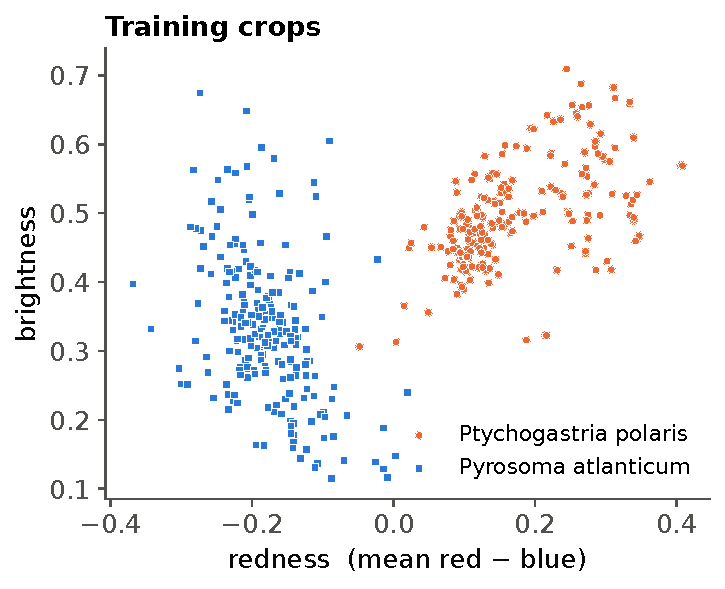
\includegraphics[width=\linewidth]{figures/two_features.pdf}
\column{0.47\textwidth}
\small
\begin{itemize}
  \item \textcolor{coral}{$\bullet$} \emph{Ptychogastria polaris}: a small reddish deep-sea jellyfish (Cnidaria)
  \item \textcolor{sea}{$\blacksquare$} \emph{Pyrosoma atlanticum}: a colonial tunicate (Chordata)
  \item every crop = one point, described by 2 numbers (\emph{features}):
  \begin{itemize}\footnotesize
    \item redness = mean (red $-$ blue) of all pixels
    \item brightness = mean grey value
  \end{itemize}
  \item \RefTwoTrain\ training crops, \RefTwoTest\ test crops
\end{itemize}
\end{columns}
\end{frame}

\begin{frame}{Be the classifier: draw a line}
\begin{columns}[c]
\column{0.5\textwidth}
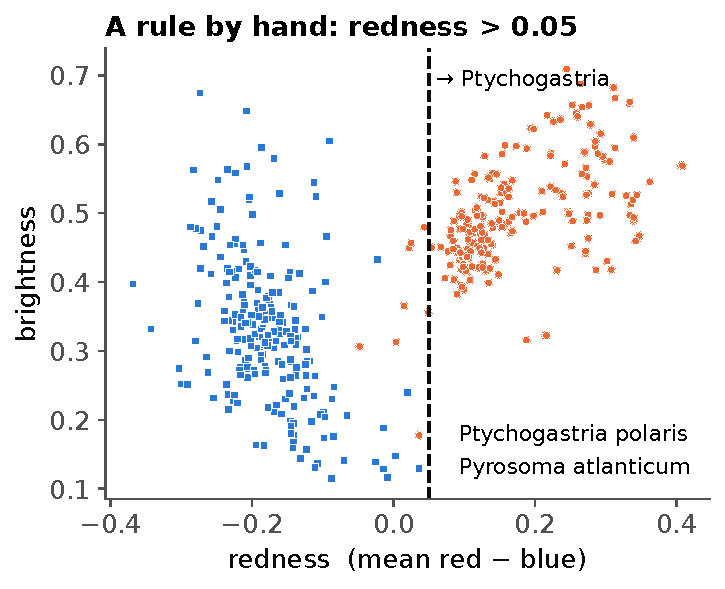
\includegraphics[width=\linewidth]{figures/two_features_threshold.pdf}
\column{0.47\textwidth}
Rule: \emph{if redness $>$ \RefThr\ then jellyfish, else tunicate.}\\[6pt]
\begin{tabular}{@{}lr@{}}
\toprule
training crops correct & \RefThrTrain \\
test crops correct & \RefThrTest \\
\bottomrule
\end{tabular}

\vspace{8pt}
The line is the \hl{decision boundary}. Everything on one side gets one label.\\[4pt]
\muted{\small In Lab 1 you choose the threshold yourself.}
\end{columns}
\end{frame}

\begin{frame}{Three ways a computer finds the boundary}
\begin{columns}[T]
\column{0.32\textwidth}
\centering\textbf{Nearest centroid}\\
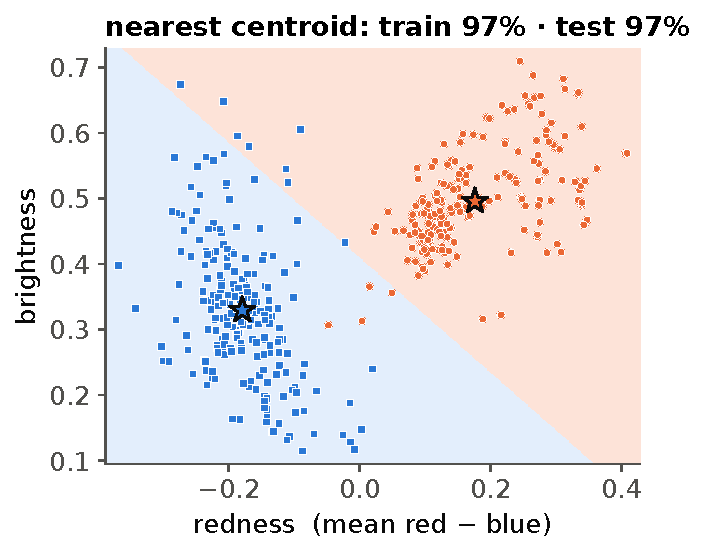
\includegraphics[width=\linewidth]{figures/boundary_centroid.pdf}\\
\small\raggedright average specimen of each label ($\star$); take the closest.\\ \muted{= the type description}
\column{0.32\textwidth}
\centering\textbf{$k$-nearest neighbours}\\
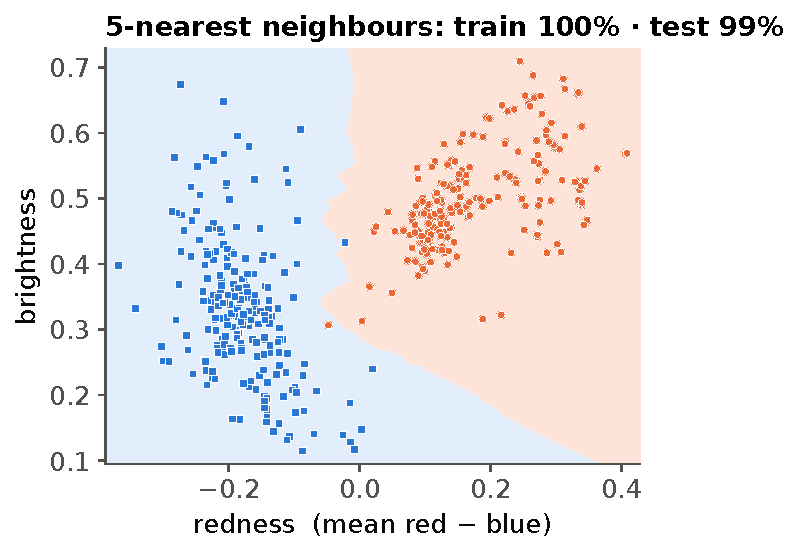
\includegraphics[width=\linewidth]{figures/boundary_knn5.pdf}\\
\small\raggedright find the $k$ most similar training crops; majority vote.\\ \muted{= the reference collection}
\column{0.32\textwidth}
\centering\textbf{Decision tree}\\
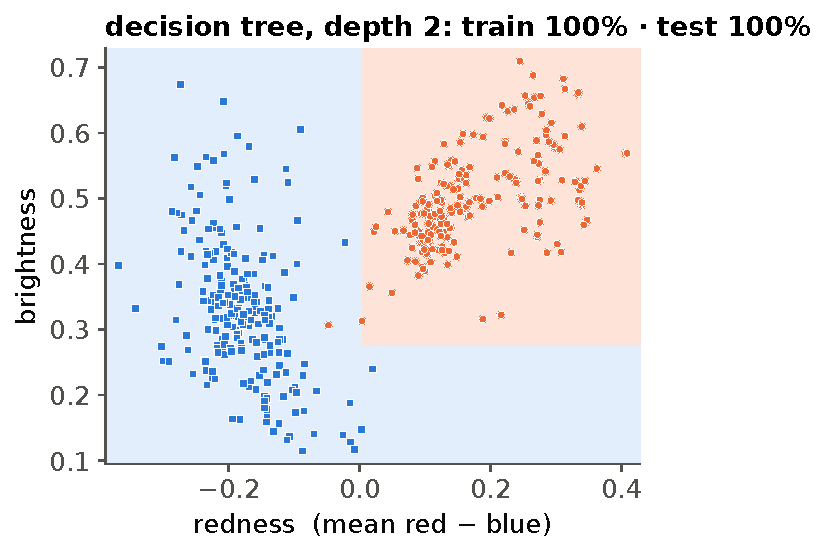
\includegraphics[width=\linewidth]{figures/boundary_tree2.pdf}\\
\small\raggedright a sequence of yes/no questions on single features.\\ \muted{= an identification key}
\end{columns}
\end{frame}

\begin{frame}{A decision tree \emph{is} an identification key}
\centering
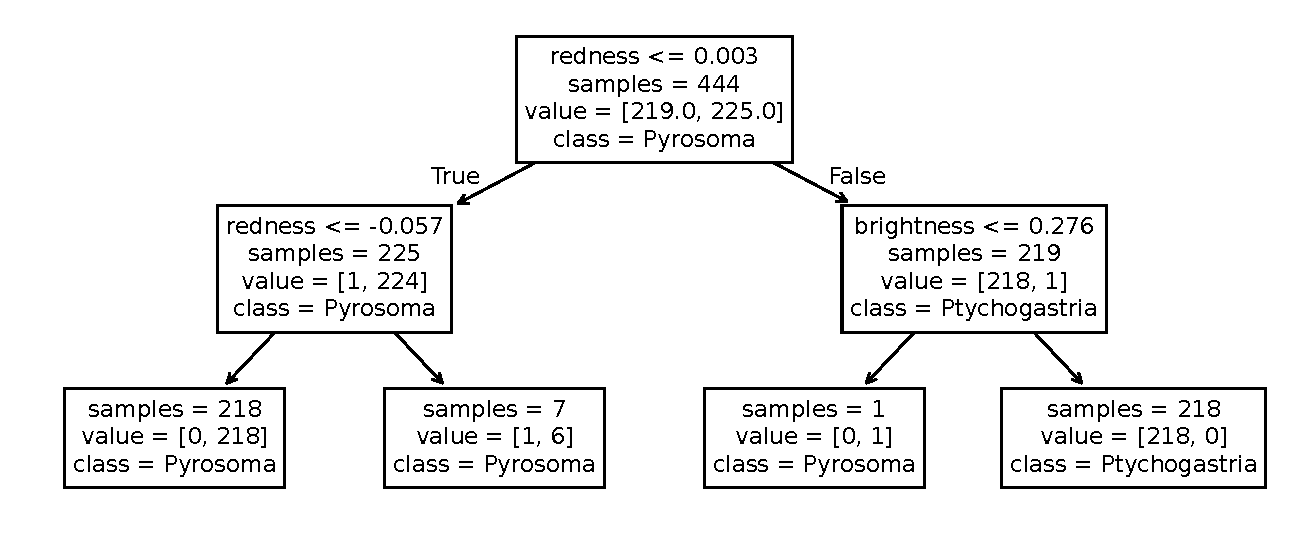
\includegraphics[width=0.78\linewidth]{figures/tree2.pdf}\\[4pt]
\small Each box: a question, how many training crops reach it (\texttt{samples}), and how they split by label (\texttt{value}).
The computer chooses the questions that separate the labels best.
\end{frame}

\begin{frame}{A harder pair: sea stars vs.\ brittle stars}
\begin{columns}[c]
\column{0.48\textwidth}
\centering\small $k=1$: copy the most similar crop\\
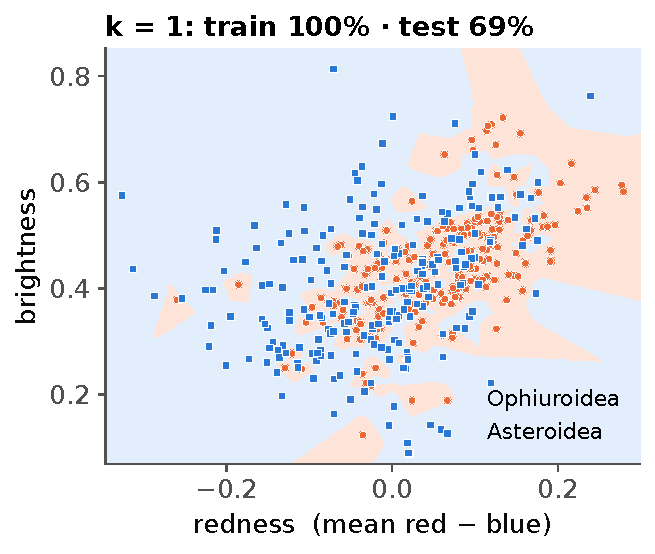
\includegraphics[height=0.52\textheight]{figures/hard_knn1.pdf}
\column{0.48\textwidth}
\centering\small $k=101$: vote of 101 neighbours\\
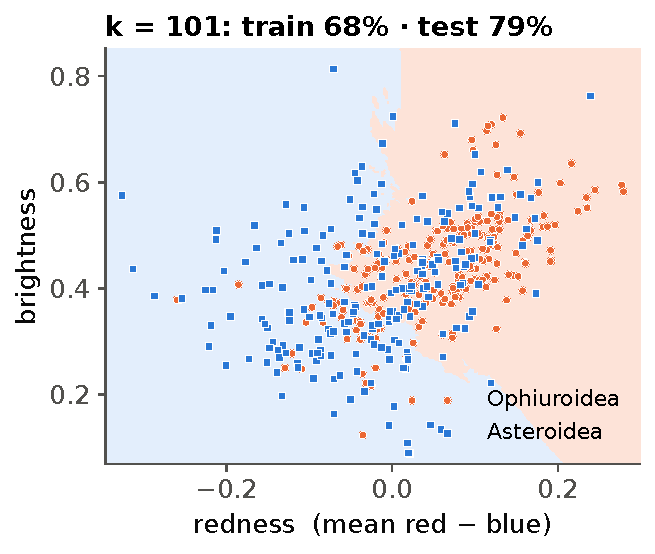
\includegraphics[height=0.52\textheight]{figures/hard_knn101.pdf}
\end{columns}
\small Colour alone does not separate Asteroidea and Ophiuroidea well. With $k=1$ the regions follow every single training crop -- 100\,\% on the training crops, but worse on the test crops.
\end{frame}

\begin{frame}{More flexible is not always better: overfitting}
\centering
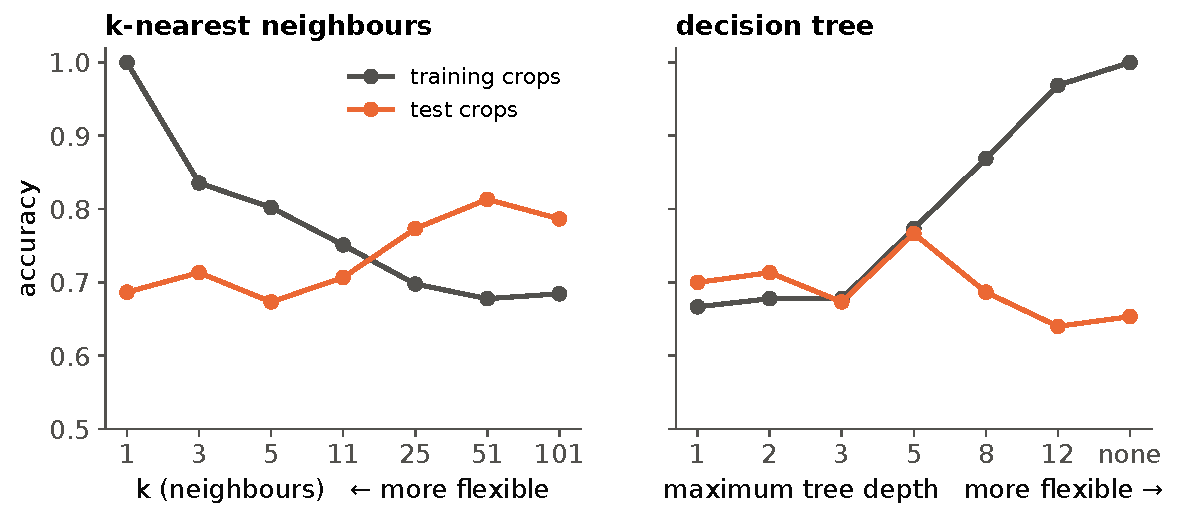
\includegraphics[width=0.8\linewidth]{figures/overfitting.pdf}\\
\small Training accuracy keeps rising when the rule gets more flexible -- test accuracy does not.
\begin{alertblock}{Overfitting}
The rule has learned the training collection \emph{by heart}, including its noise. It looks perfect on known specimens and is worse on new ones.
\end{alertblock}
\end{frame}

\begin{frame}{Rule number one: test on specimens the classifier has never seen}
\begin{columns}[c]
\column{0.55\textwidth}
\begin{tikzpicture}[>=Stealth]
  \fill[sea!25] (0,0) rectangle (4.5,1);
  \fill[coral!35] (4.5,0) rectangle (6,1);
  \node at (2.25,0.5) {\textbf{training set} (75\,\%)};
  \node at (5.25,0.5) {\textbf{test}};
  \draw[->, thick] (2.25,-0.15) -- (2.25,-0.8) node[below, align=center, font=\small] {learn the rule};
  \draw[->, thick] (5.25,-0.15) -- (5.25,-0.8) node[below, align=center, font=\small] {grade it\\(once!)};
\end{tikzpicture}
\column{0.42\textwidth}
\small
\begin{itemize}
  \item like an exam: questions must not be the practice questions
  \item training accuracy measures \emph{memory}, test accuracy measures \emph{skill}
  \item if you try many ideas, use a third part (\emph{validation set}) for choosing -- and the test set only at the very end
\end{itemize}
\end{columns}
\end{frame}

\section{The classifier zoo}

\begin{frame}{Two more classifiers, and a baseline}
\begin{description}[Logistic regression]
  \item[Baseline] ``Always say the most common label.'' Every classifier must beat it.\\
        \muted{\small With 79 equally common labels it is right $\approx$ 1 time in 79 (1.3\,\%).}
  \item[Logistic regression] A \emph{weighted checklist}: for every label, multiply each feature by a learned weight, add up $\rightarrow$ a score. Highest score wins; the scores become probabilities.
        \[ \text{score}_{\text{label}} = w_1 \cdot \text{redness} + w_2 \cdot \text{brightness} + \dots + b \]
  \item[Random forest] 300 decision trees, each built on a random part of the data. Majority vote. Much less overfitting than one tree.
  \item[Neural network] Checklists of checklists: the first layer computes new features, the next layer combines them. A CNN is a very large neural network for images.
\end{description}
\end{frame}

\begin{frame}{From 2 to 79 labels with 30 colour characters}
\begin{columns}[c]
\column{0.52\textwidth}
\small
\begin{tabular}{@{}lrr@{}}
\toprule
test accuracy & 7 phyla & 79 labels \\
\midrule
majority baseline & \RefCSPhylumMajority & \RefCSLabelMajority \\
nearest centroid & \RefCSPhylumCentroid & \RefCSLabelCentroid \\
5-nearest neighbours & \RefCSPhylumKnn & \RefCSLabelKnn \\
decision tree (depth 12) & \RefCSPhylumTree & \RefCSLabelTree \\
\bottomrule
\end{tabular}\\[3pt]
\muted{\scriptsize all 23k crops, random 75/25 split; 30 colour/texture features}
\column{0.45\textwidth}
\begin{itemize}\small
  \item 79 labels: $k$-NN is over 20$\times$ better than guessing -- colour carries information, but this is far from an expert
  \item 7 phyla: the baseline is already \RefCSPhylumMajority\ (Cnidaria is the largest phylum) -- nearest centroid is even \emph{worse} than always saying ``Cnidaria''!
\end{itemize}
\vspace{4pt}
\hl{The characters are the problem, not the rule.}\\ \small Next session: better features.
\end{columns}
\end{frame}

\begin{frame}{Lab 1 -- your first classifier}
\task{
\begin{enumerate}
  \item Choose a threshold by hand; report training and test accuracy.
  \item Compare nearest centroid, $k$-NN and a decision tree on the two features.
  \item Change $k$ and the tree depth: find where overfitting starts.
  \item Write the learned depth-2 tree as a dichotomous key.
  \item Scale up: 30 features, 7 phyla and 79 labels, compared with the baseline.
\end{enumerate}}
\vspace{4pt}
\begin{exampleblock}{Remember}
features + a rule learned from a training set $=$ classifier $\cdot$ judge it only on a test set $\cdot$ always compare with a baseline
\end{exampleblock}
\end{frame}
\end{document}
